\documentclass[11pt,]{article}
\usepackage[left=1in,top=1in,right=1in,bottom=1in]{geometry}
\newcommand*{\authorfont}{\fontfamily{phv}\selectfont}
\usepackage[]{mathpazo}


  \usepackage[T1]{fontenc}
  \usepackage[utf8]{inputenc}



\usepackage{abstract}
\renewcommand{\abstractname}{}    % clear the title
\renewcommand{\absnamepos}{empty} % originally center

\renewenvironment{abstract}
 {{%
    \setlength{\leftmargin}{0mm}
    \setlength{\rightmargin}{\leftmargin}%
  }%
  \relax}
 {\endlist}

\makeatletter
\def\@maketitle{%
  \newpage
%  \null
%  \vskip 2em%
%  \begin{center}%
  \let \footnote \thanks
    {\fontsize{18}{20}\selectfont\raggedright  \setlength{\parindent}{0pt} \@title \par}%
}
%\fi
\makeatother




\setcounter{secnumdepth}{3}

\usepackage{longtable,booktabs}

\usepackage{graphicx,grffile}
\makeatletter
\def\maxwidth{\ifdim\Gin@nat@width>\linewidth\linewidth\else\Gin@nat@width\fi}
\def\maxheight{\ifdim\Gin@nat@height>\textheight\textheight\else\Gin@nat@height\fi}
\makeatother
% Scale images if necessary, so that they will not overflow the page
% margins by default, and it is still possible to overwrite the defaults
% using explicit options in \includegraphics[width, height, ...]{}
\setkeys{Gin}{width=\maxwidth,height=\maxheight,keepaspectratio}

\title{Ecología numérica de la familia Myrtaceae en la parcela permanente de
50-ha en Barro Colorado, lago Gatún, Panamá\\
Subtítulo\\
Subtítulo  }



\author{\Large Rosee Aurelina Féliz Méndez\vspace{0.05in} \newline\normalsize\emph{Estudiante, Universidad Autónoma de Santo Domingo (UASD)}  }


\date{}

\usepackage{titlesec}

\titleformat*{\section}{\normalsize\bfseries}
\titleformat*{\subsection}{\normalsize\itshape}
\titleformat*{\subsubsection}{\normalsize\itshape}
\titleformat*{\paragraph}{\normalsize\itshape}
\titleformat*{\subparagraph}{\normalsize\itshape}

\titlespacing{\section}
{0pt}{36pt}{0pt}
\titlespacing{\subsection}
{0pt}{36pt}{0pt}
\titlespacing{\subsubsection}
{0pt}{36pt}{0pt}





\newtheorem{hypothesis}{Hypothesis}
\usepackage{setspace}

\makeatletter
\@ifpackageloaded{hyperref}{}{%
\ifxetex
  \PassOptionsToPackage{hyphens}{url}\usepackage[setpagesize=false, % page size defined by xetex
              unicode=false, % unicode breaks when used with xetex
              xetex]{hyperref}
\else
  \PassOptionsToPackage{hyphens}{url}\usepackage[unicode=true]{hyperref}
\fi
}

\@ifpackageloaded{color}{
    \PassOptionsToPackage{usenames,dvipsnames}{color}
}{%
    \usepackage[usenames,dvipsnames]{color}
}
\makeatother
\hypersetup{breaklinks=true,
            bookmarks=true,
            pdfauthor={Rosee Aurelina Féliz Méndez (Estudiante, Universidad Autónoma de Santo Domingo (UASD))},
             pdfkeywords = {Myrtaceae, Ecología numérica, mirtáceas, parcela permanente de 50-ha,
BCI},  
            pdftitle={Ecología numérica de la familia Myrtaceae en la parcela permanente de
50-ha en Barro Colorado, lago Gatún, Panamá\\
Subtítulo\\
Subtítulo},
            colorlinks=true,
            citecolor=blue,
            urlcolor=blue,
            linkcolor=magenta,
            pdfborder={0 0 0}}
\urlstyle{same}  % don't use monospace font for urls

% set default figure placement to htbp
\makeatletter
\def\fps@figure{htbp}
\makeatother

\usepackage{pdflscape} \newcommand{\blandscape}{\begin{landscape}}
\newcommand{\elandscape}{\end{landscape}}


% add tightlist ----------
\providecommand{\tightlist}{%
\setlength{\itemsep}{0pt}\setlength{\parskip}{0pt}}

\begin{document}
	
% \pagenumbering{arabic}% resets `page` counter to 1 
%
% \maketitle

{% \usefont{T1}{pnc}{m}{n}
\setlength{\parindent}{0pt}
\thispagestyle{plain}
{\fontsize{18}{20}\selectfont\raggedright 
\maketitle  % title \par  

}

{
   \vskip 13.5pt\relax \normalsize\fontsize{11}{12} 
\textbf{\authorfont Rosee Aurelina Féliz Méndez} \hskip 15pt \emph{\small Estudiante, Universidad Autónoma de Santo Domingo (UASD)}   

}

}








\begin{abstract}

    \hbox{\vrule height .2pt width 39.14pc}

    \vskip 8.5pt % \small 

\noindent El objetivo general es conocer los rasgos básicos de la estructura y
composición de la comunidad de mirtáceas en relación con factores
ambientales de la parcela permanente de 50-ha de isla Barro Colorado. Se
hicieron estudios para medir el grado de asociación, agrupamiento,
diversidad y ecología espacial de esta familia con la ayuda de los
paquetes de R y con los datos de octavo censo de esta localidad. Las
mirtáceas presentaron una riqueza de 7 especies con una abundancia de
5579 individuos. Las especies del género \emph{Eugenia} presentaron
altos grados de asociación. El agrupamiento Ward de varianza mínima
sugirió la partición de 4 grupos que alcazaron el 100\% de la
completitud de muestra. La diversidad de mirtáceas posee una correlación
positiva con \emph{Al, P, Ca, Fe} y la geomorfología de pendiente media.
Las especies \emph{Changuava schipii} y \emph{E. oerstediana} son las
especies que aportan a la diversidad alpha y están estrechamente
relacionadas con los sitios que aportan a la misma. Las mirtáceas
presentan patrones aglomerados para vecinos de primer orden, a excepción
de \emph{M. gatunencis}, que presentó un patrón aleatorio. El modelo de
abundancia de especies muestra que el 56\% de la comunidad presenta
mayores valores de equidad (log normal 10\% y null 46\%).


\vskip 8.5pt \noindent \emph{Keywords}: Myrtaceae, Ecología numérica, mirtáceas, parcela permanente de 50-ha,
BCI \par

    \hbox{\vrule height .2pt width 39.14pc}



\end{abstract}


\vskip 6.5pt


\noindent  \section{Introducción}\label{introducciuxf3n}

Uno de los temas centrales en la ecología de comunidades es cómo
controlar la diversidad alfa, es decir, el número de especies que pueden
coexistir a escalas localizadas (eg. 1 ha de una parcela). En las
plantas esta diversidad puede alcanzar niveles extraordinarios en los
bosques ecuatoriales. En el caso de los árboles, ésta en pequeños
bosques tropicales puede competir con la diversidad de árboles de los
bosques templados de todo un hemisferio. Otras formas de vida aumentan
la diversidad alfa en los bosques tropicales, especialmente las selvas
tropicales, donde los árboles representan sólo el 25\% de las especies
vegetales. Esta diversidad de las plantas es mayor en las selvas
tropicales ecuatoriales que en cualquier otro tipo de vegetación
(Wright, 2002).

La isla de Barro Colorado (BCI, por sus siglas en inglés) es un bosque
tropical, la isla se formó al término del canal de Panamá en 1914, desde
su creación se ha utilizado como centro de investigación debido a su
gran reserva natural. Se considera monumento natural protegido por el
gobierno de Panamá junto a las penínsulas Peña Blanca, Bohío, Buena
Vista, Frijoles y Gigante (Smithsonian Tropical Research Institute,
2010). La parcela permanente de 50 hectáreas se encuentra en el bosque
caducifolio húmedo tropical de la isla de Barro Colorado. Se estableció
en 1980, desde entonces se han realizado 8 censos (aprox. 1 cada 5
años), en los cuales se toman en cuenta árboles de tallos leñosos con un
diámetro a la altura del pecho (DAP) mayor a 10 mm, y como resultado en
cada censo, se han identificado, censado y mapeado más de 350,000
árboles individuales (Hubbell, Condit, \& Foster, 2021).

Las mirtáceas (Myrtaceae Juss) son una familia de plantas leñosas del
orden Myrtales, presentes en la parcela permanente de BCI. La mayoría de
las especies son árboles, también hay muchas que son arbustos o
subarbustos. Algunas especies producen flores y frutos, otras raíces
adventicias. Se distribuyen principalmente en zonas tropicales y
templadas, con poca representación en la región africana. La familia
cuenta con unos 142 géneros y más de 5.500 especies, incluyendo
\emph{Psiloxylon} y \emph{Heteropyxis}, también pueden ser citadas por
otros autores como familias monogenéricas Psiloxylaceae y
Heteropyxidaceae. Cabe destacar que la familia integra los árboles más
altos (110-140 m) del planeta (\emph{Eucalyptus}) y al género más
númeroso (1200‒1800 especies) que existe (\emph{Syzygium}), los
subarbustos rizomatosos de los géneros de la sabana (\emph{Psidium},
\emph{Campomanesia} y \emph{Eugenia}), el género \emph{Metrosideros} que
contiene especies arbóreas con muchas raíces adventicias, y otros
géneros son lianas trepadoras de raíces. También hay un mangle, el
monotípico \emph{Osbornia}, un pequeño árbol que carece de neumatóforos
(Wilson, 2010).

Las mirtaceas de BCI pertenecen a la subtribu Myrteae. Esta subtribu
posee especies que son ecológicamente importantes en muchos entornos
neotropicales debido a las bayas carnosas que comen aves y mamíferos, y
a las flores blancas generalistas que suministran polen y recursos a las
abejas. Debido a su importancia ecológica, los investigadores muestran
cada vez más interés en las Myrteae como grupo modelo para estudios
evolutivos, ecológicos y de conservación en biomas neotropicales. Cerca
del 70\% de la diversidad de especies descritas se encuentran en solo
dos géneros, \emph{Eugenia} y \emph{Myrcia}, y son dos de los géneros de
angiospermas más grandes con 1000 y 700 especies, respectivamente.
Además, se ha demostrado sistemáticamente que estos dos géneros son
hermanos de linajes pobres en especies de la tribu, lo que aumenta la
disparidad de la diversidad existente entre clados estrechamente
relacionados. La mayor parte de la biodiversidad existente de Myrteae
está restringida al Neotrópico. En el continente americano la mayor
diversidad de especies se encuentra en las selvas tropicales y la sabana
del centro, y el este de Brasil, el escudo de Guayana y el Caribe; una
biodiversidad menor, pero aún significativa, se encuentra en la América
Central continental y en la cuenca del Amazonas de tierras bajas. La
diversidad de especies es relativamente baja en las zonas subtropicales
y templadas del sur de Sudamérica (Patagonia) y en los Andes de gran
altitud, pero con una importante variedad de géneros endémicos.

En BCI, durante los repetidos censos que se han realizado en la parcela
permanente de 50-ha desde 1981 (Hubbell et al., 2021), se han reportado
varias especies de mirtáceas, siendo su representatividad relativamente
importante en dicho enclave.

Mediante análisis exploratorios preliminares, se detectaron patrones
singulares de distribución espacial y de diversidad. Algunas especies
mostraron una distribución espacial concentrada (e.g. \emph{Changuava
schipii}). Igualmente, varias especies mostraron preliminarmente
asociación con variables de suelo y geomorfólógicas. Ninguna
investigación ha reportado ni analizado estos patrones a la fecha. El
objetivo de este estudio es caracterizar la comunidad de mirtáceas de
BCI, con ayuda de técnicas de ecología numérica (e.g.~análisis de
asociación, agrupamiento, diversidad y ecología espacial en relación a
factores ambientales), utilizando como fuente los datos disponibles del
censo número de 8 de la parcela permanente de 50-ha.

\section{Metodología}\label{metodologuxeda}

\subsection{Preguntas de
investigación}\label{preguntas-de-investigaciuxf3n}

Medición de asociación: ¿Se detectan especies asociadas dentro de las
mirtaceas de BCI? ¿Existe asociación entre variables
ambientales/atributos? ¿Cuáles variables?

Agrupamiento: Los cuadros (o quadrats) de 1 hectárea, ¿se organizan en
grupos discontinuos según la composición de las especies de mirtáceas?
Si existe algún patrón, ¿es consistente con alguna variable
ambiental/atributo? ¿Hay especies indicadoras o con preferencia por
determinadas condiciones ambientales/atributos?

Diversidad: Según los análisis de estimación de riqueza, ¿están
representadas suficientemente las mirtáceas en la parcela permanente de
50-ha de BCI? ¿Existe asociación de la diversidad alpha con variables
ambientales/atributos? ¿Con cuáles? ¿Existe contribución local o por
alguna especie a la diversidad beta?

Ecología espacial: ¿Alguna(s) especies de mirtáceas presenta(n) patrón
aglomerado? ¿Cuál(es)? ¿Se asocia con alguna variable? ¿Predicen bien la
ocurrencia de dicha(s) especie(s) los modelos de distribución de
especies (SDM)?

\subsection{Ámbito geográfico}\label{uxe1mbito-geogruxe1fico}

Los datos analizados fueron colectados en la parcela permanente de 50
hectáreas de la isla Barro Colorado (BCI en lo adelante). La parcela
está situada en la meseta central de la isla (latitud 9\(^\circ\)~9'N,
longitud 79\(^\circ\)~51'O), y fue establecida en 1980 por Stephen
Hubbell y Robin Foster. Posee 1,000 m de largo por 500 m de ancho, se
divide en 1250 cuadrantes de 20x20 m (ver figura
\ref{fig:mapa_cuadros_bci}). En la parcela, todos los tallos leñosos con
un diámetro a la altura de pecho (DAP) mayor o igual a 1 cm se
encuentran marcados, enumerados, mapeados e identicados hasta el nivel
de especie. Cada 5 años, esta parcela es censada para evaluar el
crecimiento, la mortalidad y para el reclutamiento de nuevas
generaciones de plantas. Como resultado de estos censos se han
registrado mas de 300 especies de árboles, arbustos y palmas con el
próposito de conocer la historia de vida de las especies, interacciones
y dinámica de la comunidad (Pérez et al., 2005).

\begin{figure}
\centering
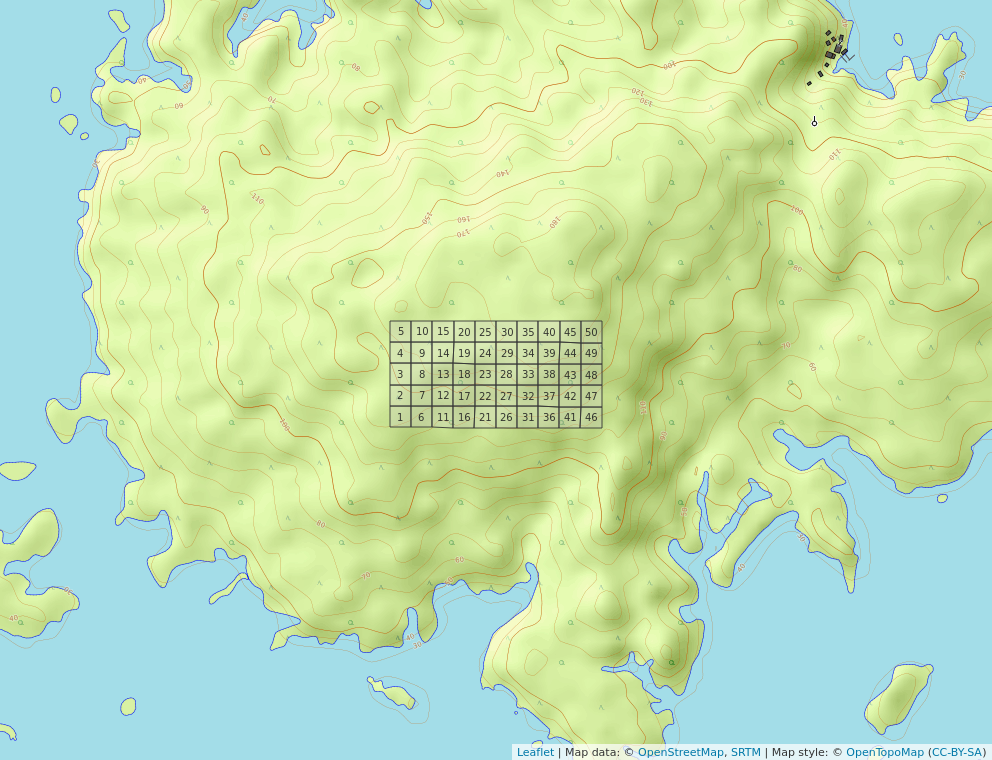
\includegraphics[width=0.50000\textwidth]{mapa_cuadros.png}
\caption{Parcela permanente de 50-ha dela isla Barro Colorado, lago
Gatún, Panamá \label{fig:mapa_cuadros_bci}}
\end{figure}

\subsection{Materiales y Métodos}\label{materiales-y-muxe9todos}

Se ha seleccionado el censo número 8 de esta reserva natural por ser el
más reciente y a esta reserva natural en particular debido a la gran
cantidad disponible de datos censales que a través de la Ecología
numérica que nos permitirán conocer rasgos básicos de la estructura y
composición de la comunidad de plantas mirtáceas en relación con
factores ambientales.

Se exploraron los datos del censo número 8 disponibles en la página web
del censo (Hubbell et al., 2021), organizados en dos matrices: la matriz
de comunidad, la cual recopila la información referente a las especies
de la parcela permanente de 50-ha, y la matriz ambiental, que contiene
la información referente a las variables de suelo, geomorfológicas,
litológicas y de tipo de habitat. Los análisis, tablas, figuras y
gráficos se realizaron con los scripts de análisis de José R. Martínez
(Batlle, 2020) y con ayuda de los paquetes de R para análisis
estadísticos y ecológicos (R Core Team, 2019), cabe destacar los
paquetes \texttt{vegan} (Oksanen et al., 2019), \texttt{tidyverse}
(Wickham, 2017), \texttt{sf} (Pebesma, 2018), \texttt{mapview}
(Appelhans, Detsch, Reudenbach, \& Woellauer, 2019) y \texttt{leaflet}
(Cheng, Karambelkar, \& Xie, 2018) que fueron los más utilizados.

En los análisis de medición de asociación en modo Q, se utilizaron
varias distancias, como ji-cuadrado, normalizada, Hellinger y Jaccard.
Las tres primeras son distancias euclideas, calculadas sobre los datos
transformados, apropiadas tanto para los datos cuantitativos como para
los datos de presencia-ausencia; y la última, la distancia de Jaccard
(\(D_J\)) se puede expresar como la proporción de especies no
compartidas. La distancia de Jaccard es el complemento a 1 de la
similaridad de Jaccard (\(S_J\)), es decir, \(D_J\) = 1- \(S_J\) , de
esta manera para obtener la similaridad, sólo hay que restarle el valor
de distancia a 1 (\(S_J\) = 1- \(D_J\)). Se puede usar para evaluar la
distancia entre especies, usando como fuente la matriz de comunidad
transpuesta convertida a binaria (presencia / ausencia) (Borcard, 2018).

Para el análisis de medición de asociación en modo R se utilizó el
coeficiente de correlación de Pearson, el cual tiene como objetivo medir
la fuerza o grado de asociación entre dos variables aleatorias
cuantitativas que poseen una distribución normal bivariada conjunta.
Alternativamente cuando este no cumple con los supuestos se utiliza
coeficiente de correlación no paramétrico de Spearman, se define como el
coeficiente de correlación lineal entre los rangos Ri(x) y Ri(y)
(Restrepo \& González, 2007).

Se realizaron análisis de agrupamiento utilizando distintos métodos
(e.g.~UPGMA, Ward) para explorar la estructura de la comunidad en
función de su composición. Para elegir entre métodos se utilizó la
correlación cofenética; se consideró al agrupamiento con la correlación
más alta como aquel que retiene la mayor parte de la información
contenida en la matriz de disimilitud; no obstante, esto no significa
necesariamente que este método sea el más adecuado para el objetivo del
investigador. Luego para escoger una cantidad óptima de clusters para
cada agrupamiento se utilizó la anchura de la silueta, ésta es una
medida del grado de pertenencia de un objeto a su clúster, basada en la
disimilitud media entre este objeto y el clúster al que pertenece,
comparada con la misma medida del clúster más próximo (Borcard, 2018).

Los métodos aglomerativos utilizados para constatar y evaluar los grupos
que hacían sentido para las mirtáceas de este estudio son desarrollados
a continuación:

-El método aglomerativo por enlace simple (\emph{single}), conocido como
la clasificación por vecinos más cercanos, aglomera objetos en función
de sus disimilitudes más cortas entre pares: la fusión de un objeto con
un grupo en un nivel de disimilitud determinado sólo requiere que un
objeto de cada grupo que se aglomerare esté vinculado al otro en ese
nivel. En consecuencia, el dendrograma resultante de una aglomeración de
enlace simple suele mostrar encadenamiento de objetos. La lista de las
primeras conexiones que hacen a un objeto miembro de un clúster, o que
permite la fusión de dos clústeres, se denomina cadena de conexiones
primarias; esta cadena forma el árbol de expansión mínima (MST).

-El método aglomerativo por enlace completo (\emph{complete}), conocido
como la clasificación del vecino más lejano, permite que un objeto se
agrupe con otro grupo sólo en la disimilitud correspondiente a la del
par de objetos más distante; de esta manera con mayor motivo, todos los
miembros de los dos grupos están vinculados. Un grupo admite un nuevo
miembro sólo a una disimilitud correspondiente al objeto más lejano del
grupo. De ello se deduce que cuánto más grande es un grupo, más difícil
es aglomerarse con él. La vinculación completa resulta en muchos grupos
pequeños separados que se aglomeran a grandes distancias, por lo que
este método es interesante para buscar e identificar discontinuidades en
los datos.

-El método de grupos de pares no ponderados con media aritmética (UPGMA,
por sus siglas en inglés) es el más conocido de la familia métodos
aglomerativos por enlace promedio, éstos se basan en las disimilitudes
medias entre los objetos o en los centroides de los grupos. El método
UPGMA permite que un objeto se una a un grupo en la media de las
disimilitudes entre este objeto y todos los miembros del grupo. Cuando
dos grupos se unen, lo hacen a la media de las disimilitudes entre todos
los miembros de un grupo y todos los miembros del otro.

-El método de agrupación de varianza mínima de Ward se basa en el
criterio del modelo lineal de mínimos cuadrados. Su objetivo es definir
los grupos de tal manera que la suma de cuadrados dentro del grupo (es
decir, el error cuadrático del ANOVA) se minimiza. La suma de errores al
cuadrado dentro del grupo puede calcularse como la suma de las
distancias al cuadrado entre los miembros de un grupo dividido por el
número de objetos. Este método fue seleccionado porque produce grupos
con números de elementos más equilibrados, o que evita los grupos de
pocos elementos (Borcard, 2018).

El remuestreo \emph{bootstrap} consiste en muestrear aleatoriamente
subconjuntos de los datos y calcular la agrupación en estos
subconjuntos. Luego de repetir este proceso un gran número de veces, se
cuenta la proporción de los resultados de clustering replicados en los
que aparece un cluster determinado. Esta proporción se denomina
probabilidad \emph{bootstrap} (BP) del cluster. Adicionalmente, se
aplicó el remuestreo \emph{bootstrap} multiescalar, utiliza muestras
\emph{bootstrap} de varios tamaños diferentes para estimar el valor p de
cada conglomerado. Esta mejora produce valores p ``aproximadamente
insesgados'' (AU) (Borcard, 2018).

Para evaluar homogeneidad de promedios de las variables ambientales
entre los grupos Ward y las variables ambientales fueron ANOVA, que
evalúa homogeneidad de medias, y Kruskal-Wallis, que evalúa la
homogeneidad de medianas; los cuales hacen sentido para agrupamientos de
3 grupos o más (Batlle, 2020).

El análisis de especies indicadoras de los grupos Ward se hizo mediante
el método del Valor Indicador (en lo adelante, IndVal), el cual se
calcula como el producto de la especificidad de una especie para el
grupo objetivo por su fidelidad al grupo objetivo. La especificidad se
define por la abundancia media de la especie dentro del grupo objetivo
comparada con su abundancia media en todos los grupos; la fidelidad es
la proporción de sitios del grupo objetivo en el que está presente la
especie. Y el análisis de especies con preferencia por hábitat se
realizó mediante el coeficiente de correlación biserial puntual
(Borcard, 2018).

Para medir la diversidad alpha se utilizaron los índices de diversidad,
descritos a continuación:

-La equidad de Pielou (denominada también equidad de Shannon) equivale a
\(J=H_1/H_0\).

-Los tres primeros números de diversidad de Hill : \(N_0 =q\) (la
riqueza de especies), \(N_1 = e^H\) (número de especies abundantes), y
\(N_1 = 1/\)\(\lambda\) (inverso de Simpson).

-Los ratios de Hill: \(E_1 = N_1/N_0\) (versión de la equidad de
Shannon) y \(E_2 = N_2/N_0\) (versión de la equidad de Simpson)
(Borcard, 2018).

La equidad puede relacionarse con la forma de los modelos de abundancia
de especies, estos son funciones que describen la forma de los gráficos
de rango/abundancia en los que la abscisa clasifica las especies en
orden de abundancia decreciente y la ordenada representa las abundancias
transformadas en logaritmos. Los cuatro modelos principales son las
series geométricas, logarítmicas y lognormales, y el modelo de barra
rota. En este orden, la uniformidad aumenta de un modelo a otro en esta
secuencia (Borcard, 2018).

Para estimar la riqueza se utilizaron los modelos de enfoque asintótico:
a) paramétricos: Modelo homogéneo (estándar y MLE), este asume que todas
las especies tienen las mismas probabilidades de incidencia o detección;
y no paramétricos: Chao1, el cual utiliza las frecuencias de únicos y
duplicados para estimar el número de especies no detectadas, Chao1-bc
(forma corregida de sesgo para el estimador Chao1) e iChao1 (estimador
Chao1 mejorado); ICE (Estimador de cobertura basado en la incidencia) e
ICE-1 (ICE modificado para casos altamente heterogéneos); Jackknife de
primer orden, el cual utiliza la frecuencia de los ejemplares únicos
para estimar el número de especies no detectadas y jackknife de 2º
orden, que utiliza las frecuencias de los únicos y los duplicados para
estimar el número de especies no detectadas. Los cuales contienen un
intervalo de confianza del 95\%, para el cual se utiliza una
transformación logarítmica, de modo que el límite inferior del intervalo
resultante sea al menos el número de especies observadas (Chao et al.,
2014).

Basado en los supuestos de Whittaker, según los cuales la diversidad
beta es la variación espacial de la diversidad entre sitios dentro de un
área geográfica de interés. Existen diferentes ecuaciones para medir esa
variación. De la investigación sobre la diversidad beta dos enfoques:
(1) La diversidad beta puede interpretarse como una rotación, es decir,
el cambio direccional en la composición de la comunidad a lo largo de un
gradiente espacial, temporal o ambiental predefinido. (2) La diversidad
beta también puede definirse como la variación de la composición de la
comunidad entre unidades de muestreo, sin referencia a un gradiente
explícito. Ambos conceptos entran en el ámbito de la definición de
Whittaker (Borcard, 2018).

Para obtener la contribuciones locales a la diversidad beta (LCBD), se
calcula primero la contribución del sitio i a la diversidad beta global
es la suma (SSi) de los valores centrados y al cuadrado del sitio (o
fila) i en la matriz S: 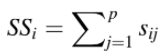
\includegraphics{beta_local.PNG}

y luego, la contribución relativa del sitio i a la diversidad beta, la
cual es denominada LCBD, es (Borcard, 2018):
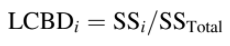
\includegraphics{beta_especies.png} donde
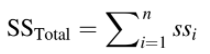
\includegraphics{beta_local2.PNG}

Para conocer las contribuciones de las especies a la diversidad beta
(SCBD), se calcula la contribución de la especie j a la diversidad beta
global es la suma (SSj) de los valores centrados y al cuadrado de la
especie (o columna) j en la matriz S:
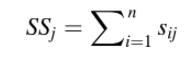
\includegraphics{beta_especies1.PNG}

y luego, la contribución relativa de la especie j a la diversidad beta,
que eso que se conoce como SCBD, es (Borcard, 2018):
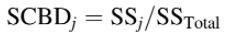
\includegraphics{beta_especies2.PNG} donde
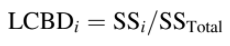
\includegraphics{beta_especies.png}

Para para explorar patrones espaciales de las especies y las variables
ambientales, se utilizaron tanto el correlograma, como la prueba Mantel,
el índice de autocorrelación I de Moran y los mapas de indicadores
locales de autocorrelación espacial (en lo adelante Mapas LISA). Serán
descritos a continuación.

El correlograma es un gráfico de los valores de correlación espacial
frente a las clases de distancia, que combinado con pruebas
estadísticas, un correlograma permite evaluar rápidamente el tipo y el
alcance de la estructura de correlación espacial de una variable
(Borcard, 2018).

El Índice Global de Moran es un analisis estadístico que examina de
forma integral las variaciones de la autocorrelación espacial entre
valores vecinos más cercanos, que se clasifican como positivo, negativo
y sin autocorrelación espacial. Cuando los valores tienden a agruparse
se trata de una autocorrelación espacial positiva, pero si se dispersan,
es una autocorrelación negativa, y si se distribuyen de forma aleatoria,
se habla de que no hay autocorrelación espacial entre los valores
analizados(Bucheli, 2019). Se construye de la siguiente manera (Borcard,
2018): 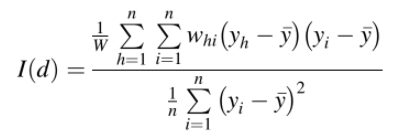
\includegraphics{moran1.PNG}

La correlación espacial en el ámbito multivariante puede evaluarse y
comprobarse mediante un correlograma de Mantel. Básicamente, se calcula
un estadístico de Mantel estandarizado rM (análogo al coeficiente r de
Pearson) entre una matriz de disimilitud entre sitios y una matriz donde
los pares de sitios que pertenecen a la misma clase de distancia reciben
el valor 0 y los demás pares, el valor 1. El proceso se repite para cada
clase de distancia. Cada valor de rM puede probarse mediante
permutaciones. La expectativa del estadístico de Mantel para la ausencia
de correlación espacial es rM \(1/4\) 0 (Borcard, 2018).

El Índice Local de Asociación Espacial (LISA) ayuda a identificar
patrones locales de asociación espacial, descomponiendo el Índice Moran
para evaluar la influencia de hábitats localizados en la estadística
global, esto se visualiza utilizando los Sistemas de Información
Geográfica. Este índice destaca las localizaciones con valores
estadísticos significativos en los indicadores, resaltando la presencia
de puntos calientes \emph{hot spots} o atípicos espaciales, dependiendo
de los datos estadísticos analizados. El resultado es la la generación
de un mapa que se denomina de agrupamiento o clúster, en este se
visualiza cada unidad espacial se diferenciada de sus unidades vecinas
(Bucheli, 2019).

\section{Resultados}\label{resultados}

La familia Myrtaceae de la parcela permanente de 50-ha de BCI presentó
una abundancia de 5,579 individuos pertenecientes a 7 especies, de las
cuales las más abundantes fueron \emph{Eugenia galalonensis} y
\emph{Eugenia oerstediana}, representadas con 1,975 y 1,838 individuos
cada una, y las especies más raras fueron \emph{Psidium
friedrichsthalianum} y \emph{Myrcia gatunensis}, con 58 y 56 individuos
respectivamente (ver figura \ref{tab:abun_sp}).

\begin{longtable}[]{@{}lr@{}}
\caption{\label{tab:abun_sp}Abundancia por especie de la familia
Myrtaceae}\tabularnewline
\toprule
Latin & n\tabularnewline
\midrule
\endfirsthead
\toprule
Latin & n\tabularnewline
\midrule
\endhead
Eugenia galalonensis & 1975\tabularnewline
Eugenia oerstediana & 1838\tabularnewline
Eugenia coloradoensis & 609\tabularnewline
Chamguava schippii & 541\tabularnewline
Eugenia nesiotica & 502\tabularnewline
Psidium friedrichsthalianum & 58\tabularnewline
Myrcia gatunensis & 56\tabularnewline
\bottomrule
\end{longtable}

\begin{figure}
\centering
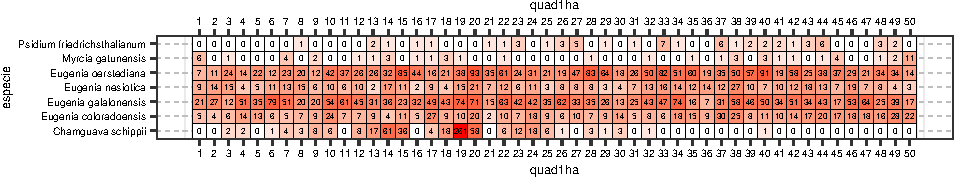
\includegraphics{manuscrito_files/figure-latex/unnamed-chunk-3-1.pdf}
\caption{\label{fig:abun_sp_q}Abundancia de especies por quadrat}
\end{figure}

Para los análisis de medición de asociación, la distancia de
\emph{ji}-cuadradado y la distancia de Jacard resultaron pequeñas entre
especies del genéro \emph{Eugenia} (\emph{E. oerstediana}, \emph{E.
galalonensis}, \emph{E. nesiotica} y \emph{E. coloradoensis}), lo cual
sugiere un patrón de dependencia, debido a que tienen altos grados de
asociación; y las especies \emph{Psidium friedrichsthalianum},
\emph{Myrcia gatunensis} y \emph{Changuava schippii} presentan un
posible patrón independiente, no parecen asociarse con otras (ver figura
\ref{fig:matriz_Jacard}). La riqueza de la familia presentó asociación
estadística, a través del índice de Spearman, en términos positivos con
\emph{Al}, * P* y en términos negativos con \emph{Ca}; y la abundancia
de mi familia presentó asociación estadística, a través del índice de
Spearman y el índice de Pearson, en términos positivos con \emph{Al} y
elevación media, y en términos negativos con \emph{Ca}, heterogeneidad
ambiental y geomorfología de vaguada (ver figuras
\ref{fig:matriz_spearman} y \ref{fig:matriz_pearson}).

\begin{figure}
\centering
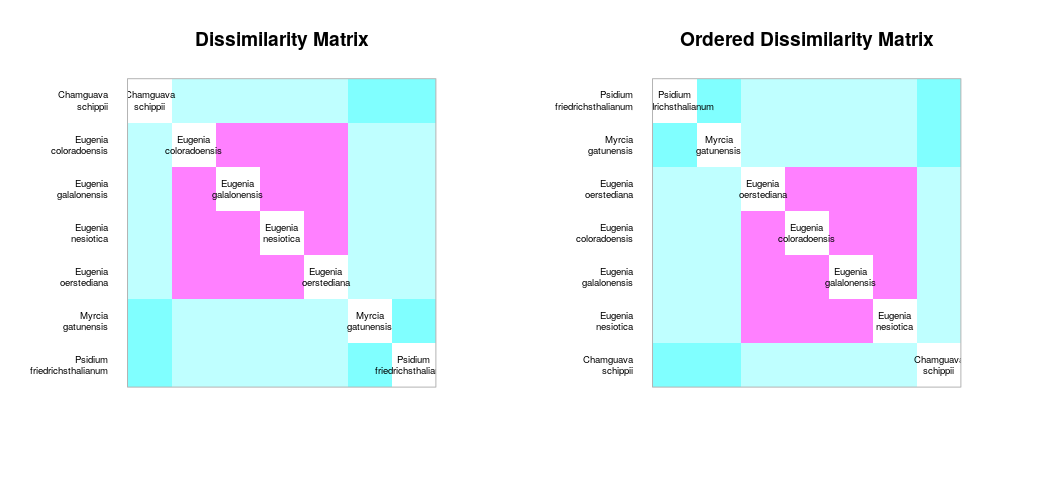
\includegraphics{Disimilaridad_.png}
\caption{Matriz de disimilaridad de Jacard \label{fig:matriz_Jacard}}
\end{figure}

\begin{figure}
\centering
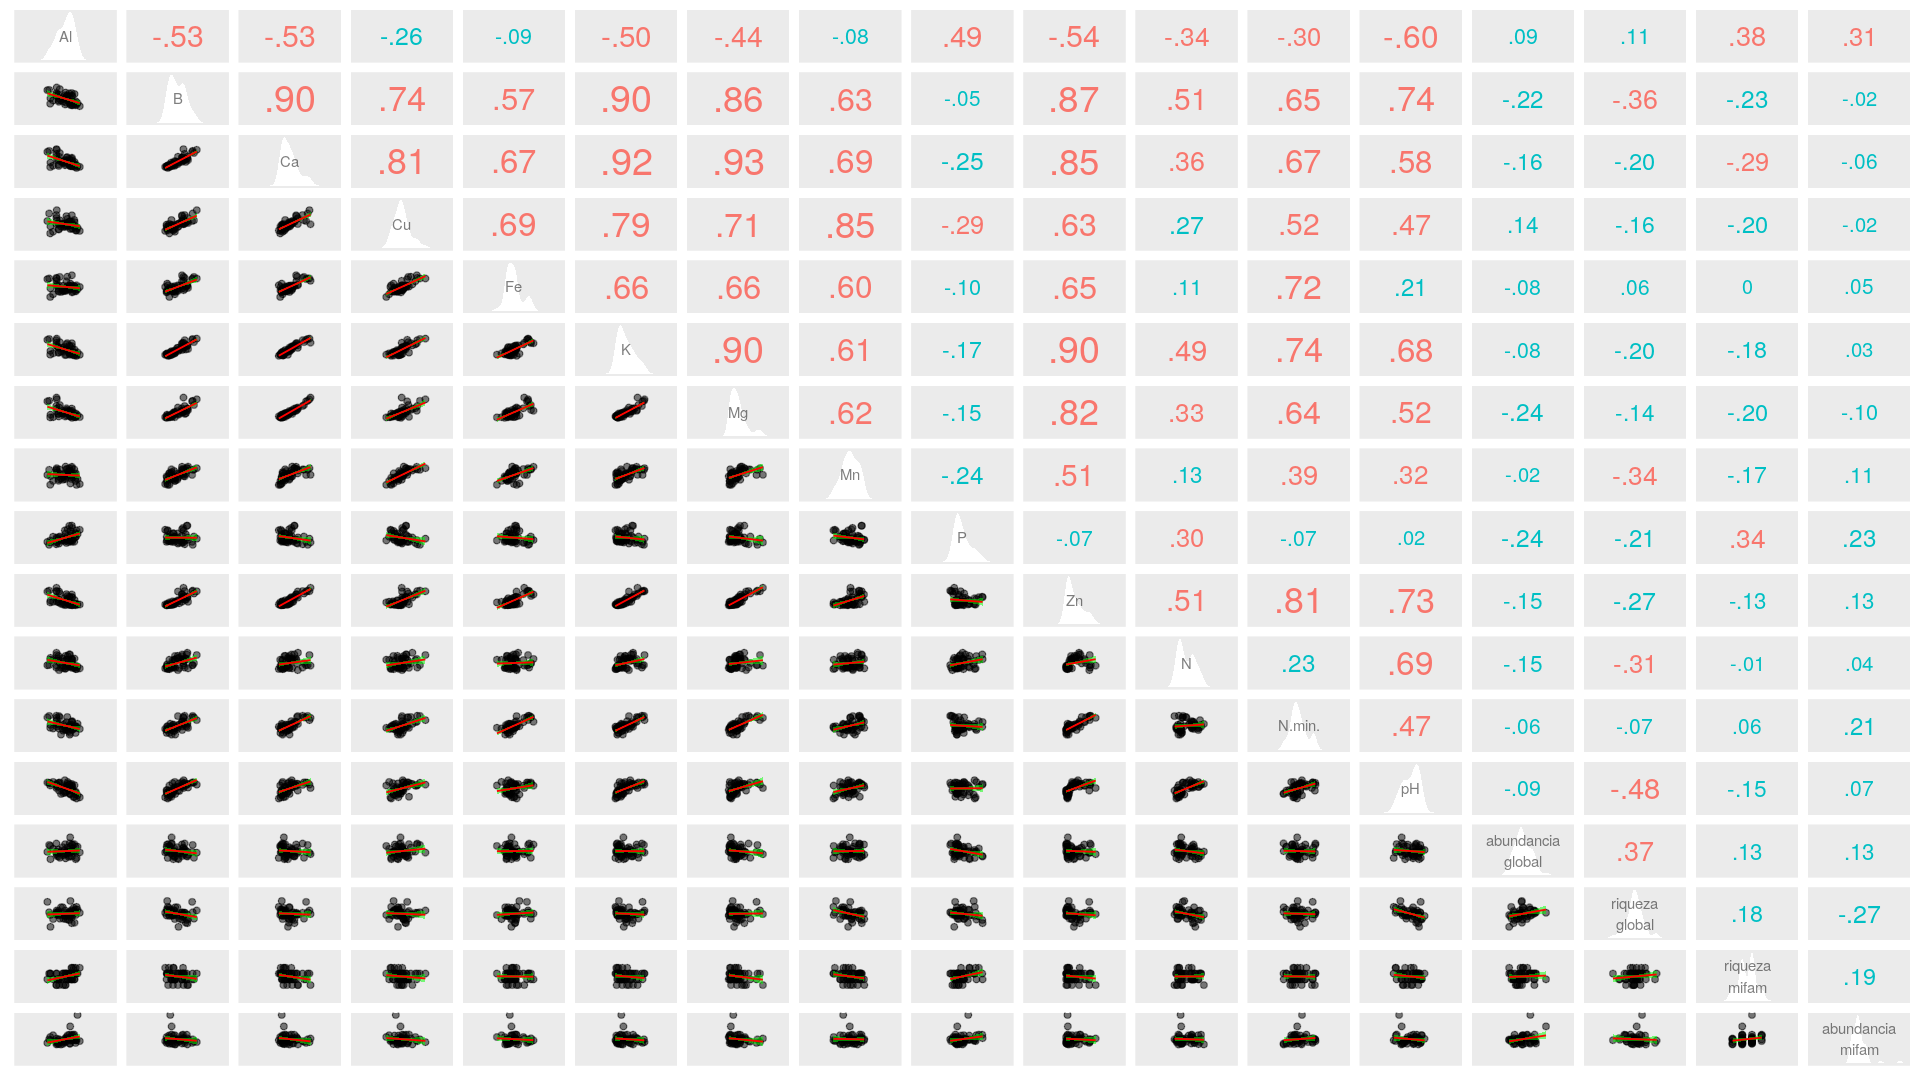
\includegraphics{matriz_correlacion_suelo_abun_riq_spearman.png}
\caption{Matriz de correlación, índice de Spearman
\label{fig:matriz_spearman}}
\end{figure}

\begin{figure}
\centering
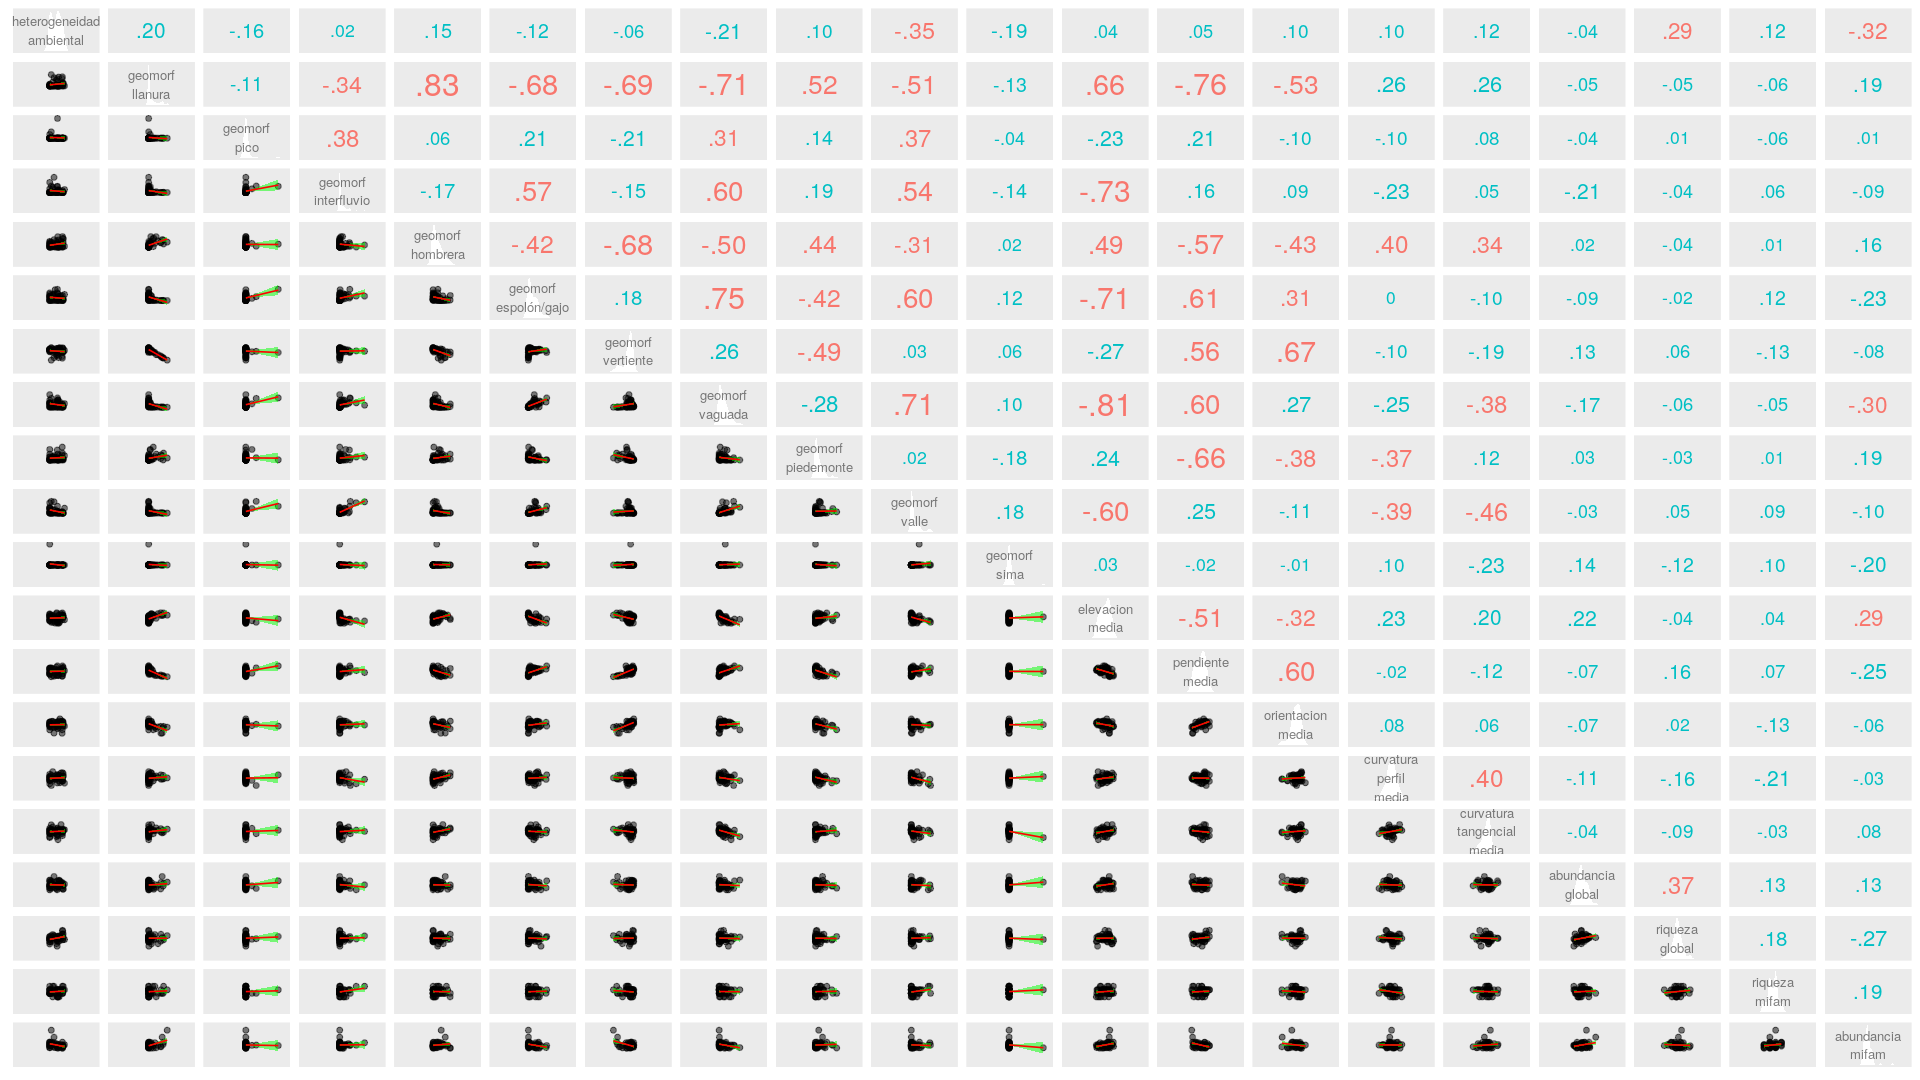
\includegraphics{matriz_correlacion_geomorf_abun_riq_spearman.png}
\caption{Matriz de correlación, índice de Pearson
\label{fig:matriz_pearson}}
\end{figure}

Para los análisis de agrupamiento (\emph{cluster analysis}), se utilizó
el método de agrupamiento Ward de varianza mínima, conjuntamente con el
mapa de calor (ver figuras \ref{fig:mapadecalor_ward} y
\ref{fig:ward_fraccionado}), los cuales mostraron que las mirtáceas de
la parcela permanente de 50-ha de BCI se distribuyen en 4 grupos, de 2,
13, 15 y 20 sitios, respectivamente (ver figura \ref{fig:mapa_ward}).
Los métodos de agrupamiento aglomerativos por enlace simple, por enlace
completo y por enlace promedio (grupos de pares no ponderados con media
aritmética, UPGMA por sus siglas en inglés) destacaron la singularidad
de este grupo formado por dos sitios (14 y 19). Además, el muestreo de
\emph{bootstrap} multiescalar respaldó este grupo con un probabilidad de
\emph{bootstrap} (BP) de 76 \% y probabilidad de valores aproximadamente
insesgados (AU) de 99 \%, de que sea un grupo real (ver figura
\ref {fig:*bootstrap*_multiescalar}). Las mirtáceas presentaron
asociación estadística, según el diagrama de cajas, con un conjunto de
variables de suelo (\emph{Al, Fe, Mn, N. min.}, etc.) y atributos del
terreno (curvatura perfil media, curvatura tangencial media, elevación
media, etc.) (ver figura \ref{fig:ward_con_variables}). ANOVA,
Kruskal-Walis*

\begin{figure}
\centering
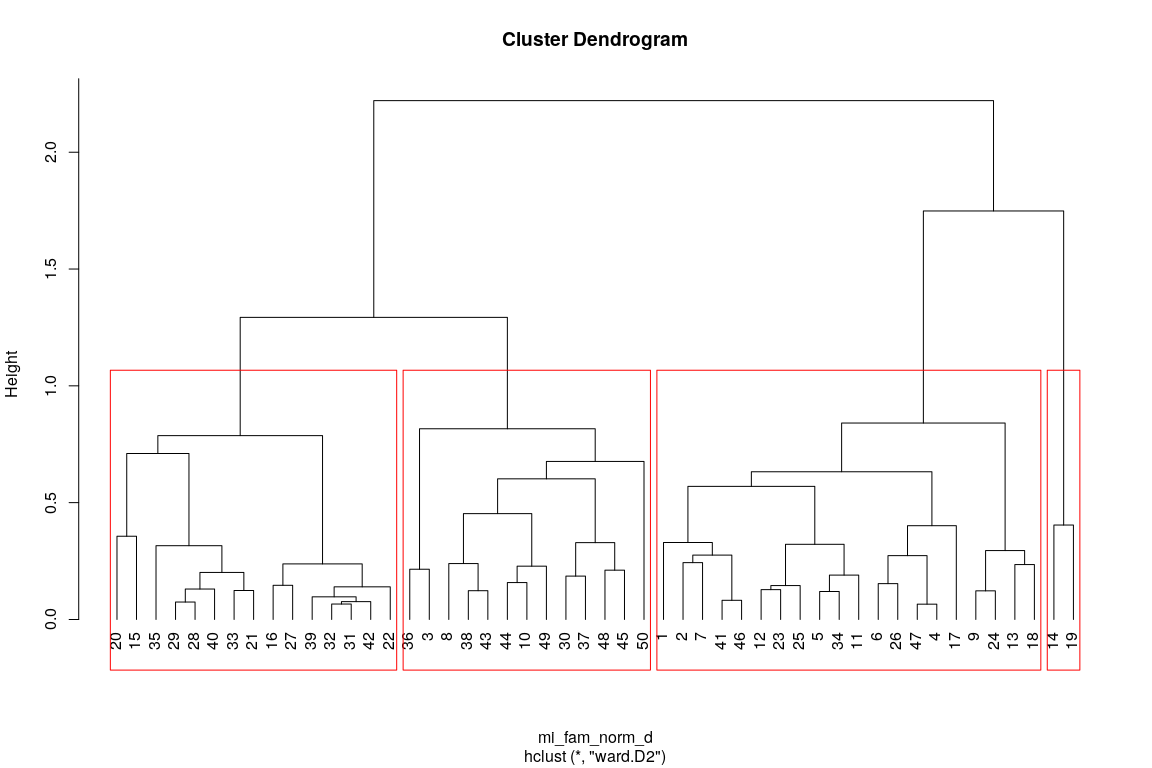
\includegraphics[width=0.50000\textwidth]{ward_fracionado.png}
\caption{Agrupamiento por el método Ward de varianza mínima de las
mirtáceas \label{fig:ward_fraccionado}}
\end{figure}

\begin{figure}
\centering
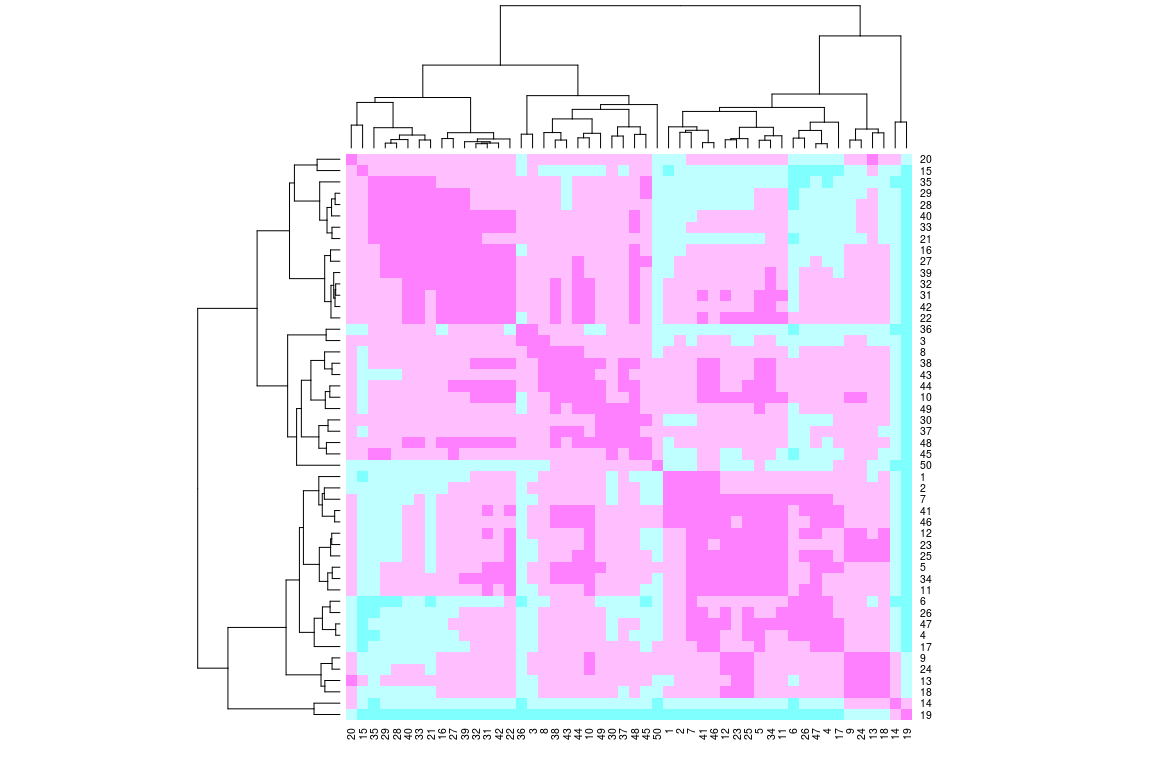
\includegraphics[width=0.50000\textwidth]{Mapadecalor_Ward_aa2.png}
\caption{Mapa de calor con el dendrograma del agrupamiento Ward
\label{fig:mapadecalor_ward}}
\end{figure}

\begin{figure}
\centering
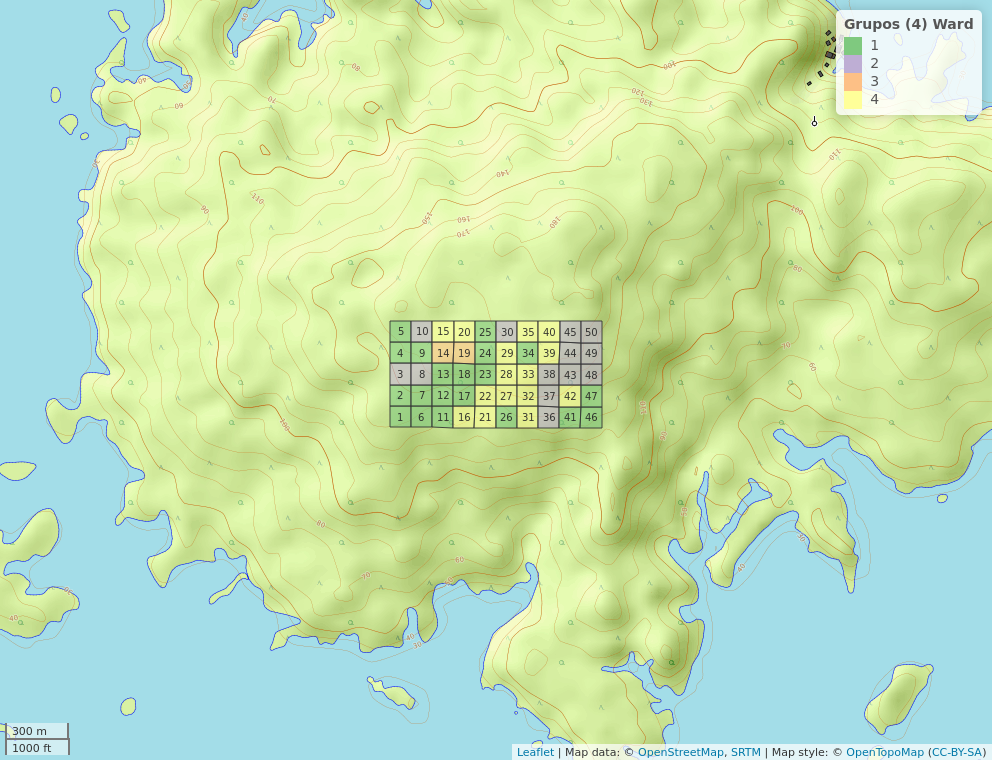
\includegraphics[width=0.50000\textwidth]{mapa_ward_k4.png}
\caption{Agrupamiento por el método Ward de varianza mínima de las
mirtáceas \label{fig:mapa_ward}}
\end{figure}

\begin{figure}
\centering
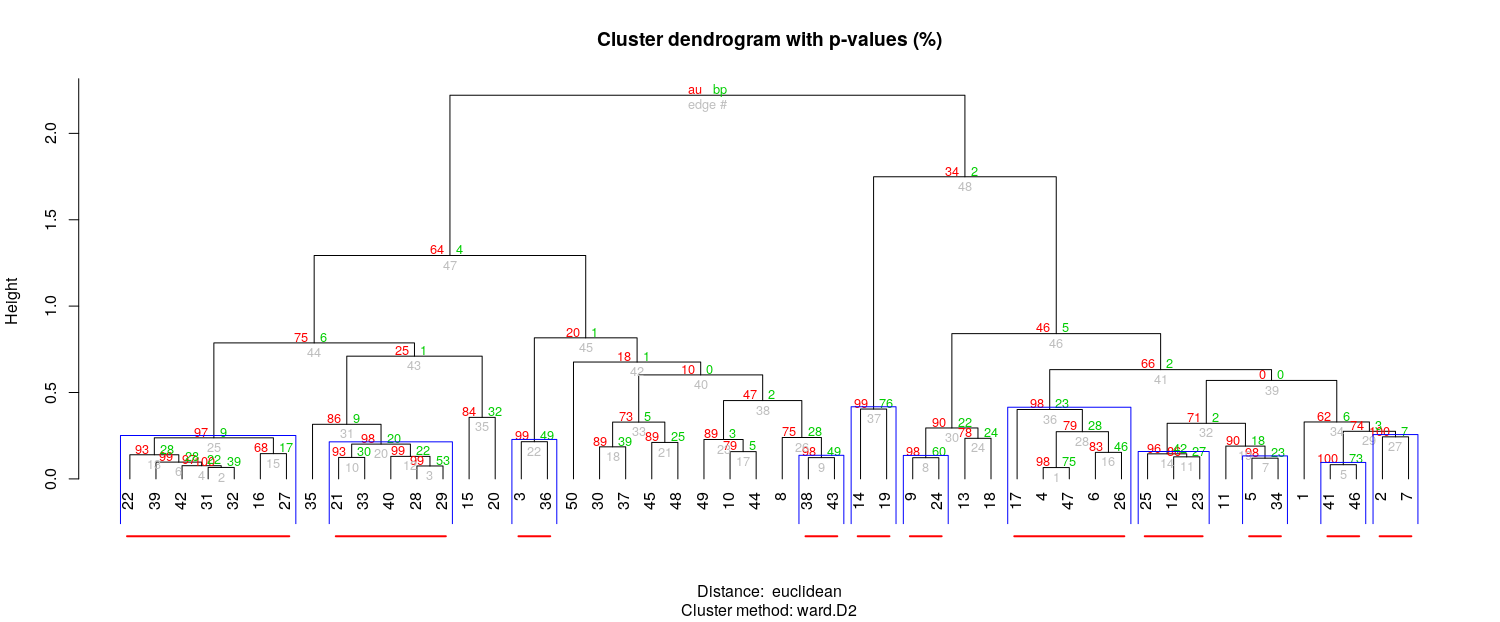
\includegraphics{bootstrap_Ward.png}
\caption{Dendrograma, agrupamiento Ward con los porcentajes del
remuestreo de \emph{bootstrap} multiescalar
\label{fig:*bootstrap*_multiescalar}}
\end{figure}

\begin{figure}
\centering
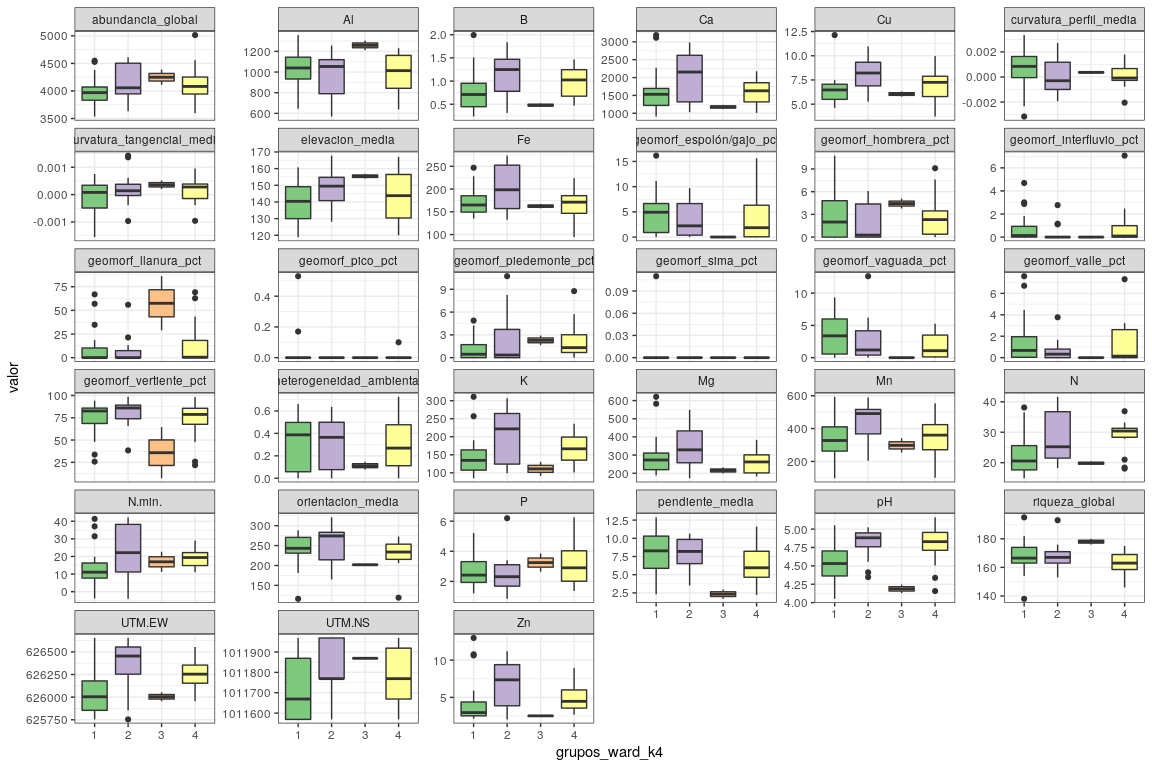
\includegraphics{correlograma_wardyvariablesambientales.png}
\caption{Diagrama de cajas de los grupos Ward en relación con variables
ambientales y atributos \label{fig:ward_con_variables}}
\end{figure}

Para este agrupamiento, las especies asociadas como indicadoras,
mediante IndVal para una significancia menor de 0.05, fueron
\emph{Chamguava schippii} para el grupo 3, \emph{Eugenia coloradoensis}
para el conjunto de grupos 1+2 y \emph{Eugenia oerstediana} para el
conjunto de grupos 3+4; y las especies con preferencia por hábitat,
mediante el coeficiente de correlación biserial puntual para una
significancia menor de 0.05, fueron \emph{Eugenia coloradoensis} con
preferencia por el grupo 2, \emph{Chamguava schippii} por el grupo 3 y
\emph{Eugenia oerstediana} por el grupo 4.

\begin{longtable}[]{@{}l@{}}
\toprule
Multilevel pattern analysis\tabularnewline
\midrule
\endhead
Association function: IndVal.g\tabularnewline
Significance level (alpha): 0.05\tabularnewline
---------------------------------\tabularnewline
Total number of species: 7\tabularnewline
Selected number of species: 3\tabularnewline
Number of species associated to 1 group: 1\tabularnewline
Number of species associated to 2 groups: 2\tabularnewline
Number of species associated to 3 groups: 0\tabularnewline
---------------------------------------------\tabularnewline
List of species associated to each combination\tabularnewline
-------------------------------------------------\tabularnewline
Group 3 \#sps. 1\tabularnewline
-------------------\tabularnewline
Chamguava schippii\tabularnewline
------------------------------------------------------\tabularnewline
Group 1+2 \#sps. 1\tabularnewline
--------------------\tabularnewline
Eugenia coloradoensis\tabularnewline
-----------------------------------------------------\tabularnewline
Group 3+4 \#sps. 1\tabularnewline
---------------------\tabularnewline
Eugenia oerstediana 0.6515\tabularnewline
\bottomrule
\end{longtable}

Signif. codes: 0 \(‘***’\), 0.001 \(‘**’\), 0.01 \(‘*’\), 0.05 `.', 0.1
`', 1

Para los análisis de diversidad, se utilizaron los modelos de estimación
de riqueza (\emph{Homogeneous model}, estándar y MLE; los Chao y los
Jacknife), los cuales mostraron que la completitud de muestra se alcanzó
al 100\% para las mirtáceas de este ámbito geográfico por lo que no
sería necesario aumentar el esfuerzo de muestreo ya que no se espera
encontrar otras especies en BCI*. La diversidad alpha para el
agrupamiento Ward, los cuatro grupos presentaban la riqueza máxima (7
especies) con diferentes abundancias (1882, 1205, 553 y 1939,
respectivamente). Para los grupos Ward, la riqueza máxima fue estimada y
observada, por lo que también se alcanzó la completitud de muestra al
100\% y al 98\% para el grupo 3 (grupo con la menor abundancia), y no
será necesario aumentar los esfuerzos de muestreo.

La riqueza (\(N_0\)), \(E_2\) y \(N_2\) de Hill mostraron que la
diversidad de mirtáceas presenta una correlación positiva importante con
\emph{Al, P, Ca y Fe}, en suma la equidad de Pielou (J), los ratios de
Hill (\(E_1\) y \(E_2\)) y \(N_2\) mostraron una correlación positiva
notable con la presencia de la geomorfología de pendiente media.

\emph{Changuava schipii} y \emph{Eugenia oerstediana} fueron las
especies que hacen contribución a la diversidad beta, éstas están bien
representadas (la primera con gran dominancia) en los sitios 14 y 19
(grupo 3 Ward) que hacen contribución a la diversidad beta; el 14 fue
uno de los cinco sitios que poseen la riqueza máxima (los demás sitios
son 13, 17, 22 y 40) y el 19 fue el sitio más abundante con 399
individuos, de los cuales 261 pertenecían a \emph{C. schipii} (ver
figura \ref{fig:abun_sp_q}). Además, los sitios 14 y 19 están ubicados
uno al lado del otro. El modelo de abundancia de especies muestra que el
56\% de la comunidad presenta mayores valores de equidad (log normal
10\% y null 46\%).

Para los análisis de ecología espacial, la prueba I de Moran sugirió que
las mirtáceas de esta localización presentaron patrones aglomerados al
menos con la vecindad de primer orden, con excepción de \emph{M.
gatunensis} y \emph{E. galalonensis} que mostraron un patrón espacial
aleatorio. Cabe destacar que \emph{C. schipii} presentó una
autocorrelación espacial positiva también para los vecinos de segundo
orden y en términos negativos del cuarto al sexto orden; para \emph{E.
nesiotica} y \emph{E. oerstediana} una autocorrelacion negativa con
vecinos de tercer a cuarto orden y de cuarto a quinto orden,
respectivamente, es decir, su abundancia disminuye en esas vecindades
cuando aumenta en la de primer orden y viceversa.

La autocorrelación mediante la prueba de Mantel muestra que hay una
correlación espacial inducida por alguna variable en términos positivos
para el primer orden y en términos negativos para el tercer y sexto
orden (hasta 500 metros). La prueba Yo de Moran evidencia que \emph{C.
schipii} muestra un posible patrón de correlación inversa con el
\emph{B, Ca, Zn, N y pH}; para \emph{E. coloradoensis} infiere un patrón
en términos positivos con \emph{Ca} y \emph{N. min.} y de igual manera
para \emph{E. galalonensis} con la geomorfología de vaguada pct y
pendiente media.

\section{Discusión}\label{discusiuxf3n}

La comunidad de mirtáceas de la parcela permante de BCI posee una
riqueza de 7 especies con una abundancia de 5579 individuos, la mayor
abundancia se registró para las especies \emph{E. galalonensis}
(35.40\%) y \emph{E. oerstediana} (32.94\%) y la menor abundancia para
las especies \emph{P. friedrichsthalianum} (1.04\%) y \emph{M.
gatunensis} (1.004\%). En cada quadrat de la parcela BCI podemos
encontrar un mínimo de 58 y un máximo de 399 mirtáceas para un promedio
de 112 individuos por quadrat.

El 57\% de la riqueza, las especies del género \emph{Eugenia},
presentaron altos grados de asociación entre ellas, por lo que supone un
patrón de dependencia, a diferencia de las especies \emph{P.
friedriechsthalianum}, \emph{M. gatunensis} y \emph{C. schipii}
mostraron un posible patrón independiente, por lo que supone que se
presentan aleatoriamente en la muestra sin asociarse a las otras
especies.

Las mirtáceas de esta muestra, según el método Ward, se dividen en 4
grupos, cada uno con 2, 13, 15 y 20 sitios respectivamente; el grupo con
2 sitios es respaldado por los métodos de agrupamiento aglomerativo y el
\emph{bootstrap} multiescalar (BP de 76\% y un AU de 99\%) esto infiere
que es un grupo natural y real dentro de la localidad. Este agrupamiento
no se relaciona específicamente con alguna variable sino por la
preferencia de un conjunto de éstas, como lo son \emph{Al} y \emph{Fe}.

Según el análisis de especies indicadoras (IndVal), las especies
asociadas como diagnósticas para el agrupamiento Ward, fueron \emph{C.
schipii} para el grupo 3, \emph{E. coloradoensis} para el conjunto 1+2 y
\emph{E. oerstediana} para el grupo 3+4, esto puede ser debido a sus
altas abundancias presentes en estos grupos.

Los estimadores de riqueza demostraron que la completitud de muestra
para las mirtáceas en estudio fue alcanzda 100\%, lo mismo para los
grupos Ward, por lo que inferimos que el esfuerzo de muestreo surtió las
necesidas de lugar y no se espera encontrar más especies de en de esta
familia en BCI.

Los equidad de Pielou, los números de Hill destacan que la diversidad de
mirtáceas posee una correlación positiva con \emph{Al, P, Ca, Fe} y la
geomorfología de pendiente media.

Las especies que hacen contribución a la diversidad beta son \emph{C.
schipii} y \emph{E. oerstediana}, y los sitios que hacen contribución a
esta diversidad son el grupo 14 y 19, coincidencialmente un grupo Ward
que posee altas abundancias de las especies antes mencionadas, por lo
que este grupo guarda una estrecha relación con la presencia de estas
especies.

Las mirtáceas de esta localidad, según el I de Moran, presentan patrones
aglomerados para vecinos de primer orden que implican hasta 50 sitios,
con excepción de \emph{M. gatunencis}, que como había mencionado antes,
presentó un patrón aleatorio; en el caso de \emph{C. schipii}, presenta
patrón más aglomerado que las demás debido a que presenta una
correlación positiva también con los vecinos de segundo orden y en
términos negativos con los vecinos del cuarto al sexto orden, es decir
que aumenta o disminuye de forma inversa en estos lugares en relación
con el primer y segundo orden.

El modelo de abundancia de especies muestra que el 56\% de la comunidad
presenta mayores valores de equidad (log normal 10\% y null 46\%),
parece una cifra razonable debido a que el 48\% de los quadrats poseen
valores 7 y 6 de riqueza, lo que infiere que los modelos de distribución
de especies (SDM) parecen estar prediciendo bien la ocurrencia de dichas
especies.

\section{Agradecimientos}\label{agradecimientos}

\section{Información de soporte}\label{informaciuxf3n-de-soporte}

\ldots

\section{\texorpdfstring{\emph{Script}
reproducible}{Script reproducible}}\label{script-reproducible}

\ldots

\section*{Referencias}\label{referencias}
\addcontentsline{toc}{section}{Referencias}

\hypertarget{refs}{}
\hypertarget{ref-mapview}{}
Appelhans, T., Detsch, F., Reudenbach, C., \& Woellauer, S. (2019).
\emph{Mapview: Interactive viewing of spatial data in r}. Retrieved from
\url{https://CRAN.R-project.org/package=mapview}

\hypertarget{ref-jose_ramon_martinez_batlle_2020_4402362}{}
Batlle, J. R. M. (2020). biogeografia-master/scripts-de-analisis-BCI:
Long coding sessions (Version v0.0.0.9000).
\url{https://doi.org/10.5281/zenodo.4402362}

\hypertarget{ref-borcard2018numerical}{}
Borcard, F. ~. ois y L., Daniel y Gillet. (2018). \emph{Ecología
numérica con r}. Springer.

\hypertarget{ref-bucheli2019uso}{}
Bucheli, G. E. H. (2019). Uso del Índice de moran y lisa para explicar
el ausentismo electoral rural en ecuador. \emph{Revista Geográfica},
(160), 91--108.

\hypertarget{ref-paqueteiNEXT}{}
Chao, A., Gotelli, N. J., Hsieh, T. C., Sande, E. L., Ma, K. H.,
Colwell, R. K., \& Ellison, A. M. (2014). Rarefaction and extrapolation
with hill numbers: A framework for sampling and estimation in species
diversity studies. \emph{Ecological Monographs}, \emph{84}, 45--67.

\hypertarget{ref-leaflet}{}
Cheng, J., Karambelkar, B., \& Xie, Y. (2018). \emph{Leaflet: Create
interactive web maps with the javascript 'leaflet' library}. Retrieved
from \url{https://CRAN.R-project.org/package=leaflet}

\hypertarget{ref-webcenso}{}
Hubbell, S., Condit, R., \& Foster, R. (2021). Forest Census Plot on
Barro Colorado Island. Retrieved May 5, 2021, from
\url{http://ctfs.si.edu/webatlas/datasets/bci/}

\hypertarget{ref-vegan}{}
Oksanen, J., Blanchet, F. G., Friendly, M., Kindt, R., Legendre, P.,
McGlinn, D., \ldots{} Wagner, H. (2019). \emph{Vegan: Community ecology
package}. Retrieved from \url{https://CRAN.R-project.org/package=vegan}

\hypertarget{ref-sf}{}
Pebesma, E. (2018). Simple Features for R: Standardized Support for
Spatial Vector Data. \emph{The R Journal}, \emph{10}(1), 439--446.
\url{https://doi.org/10.32614/RJ-2018-009}

\hypertarget{ref-perez2005metodologia}{}
Pérez, R., Aguilar, S., Condit, R., Foster, R., Hubbell, S., \& Lao, S.
(2005). Metodologia empleada en los censos de la parcela de 50 hectareas
de la isla de barro colorado, panamá. \emph{Centro de Ciencias
Forestales Del Tropico (CTFS) Y Instituto Smithsonian de Investigaciones
Tropicales (STRI)}, 1--24.

\hypertarget{ref-citadeR}{}
R Core Team. (2019). \emph{R: A language and environment for statistical
computing}. Retrieved from \url{https://www.R-project.org/}

\hypertarget{ref-restrepo2007pearson}{}
Restrepo, L. F., \& González, J. (2007). From pearson to spearman.
\emph{Revista Colombiana de Ciencias Pecuarias}, \emph{20}(2), 183--192.

\hypertarget{ref-bci_video}{}
Smithsonian Tropical Research Institute. (2010). \emph{Un vistazo a la
ciencia y los cientificos que trabajan en la isla de Barro Colorado}.
urlhttps://youtu.be/bN54RGtxFeM.

\hypertarget{ref-tidyverse}{}
Wickham, H. (2017). \emph{Tidyverse: Easily install and load the
'tidyverse'}. Retrieved from
\url{https://CRAN.R-project.org/package=tidyverse}

\hypertarget{ref-wilson2010myrtaceae}{}
Wilson, P. G. (2010). Myrtaceae. In \emph{Flowering plants. eudicots}
(pp. 212--271). Springer.

\hypertarget{ref-wright2002plant}{}
Wright, J. S. (2002). Plant diversity in tropical forests: A review of
mechanisms of species coexistence. \emph{Oecologia}, \emph{130}(1),
1--14.




\newpage
\singlespacing 
\end{document}
